%% CLIQUES
\begin{frame}
\frametitle{Método de Compresión Propuesto}

Consta de tres etapas:

\begin{enumerate}
	\item Listar todos los cliques maximales del grafo.
	\item Particionar listado de cliques, utilizando heurística eficiente que explote su superposición.
	\item Comprimir particiones en estructura compacta.
\end{enumerate}

\end{frame}


%\begin{frame}
%\frametitle{Etapa 1: Cliques Maximales}
%
%Se obtiene el listado de cliques, usando \textbf{Quick Cliques}\footnote{\url{https://github.com/darrenstrash/quick-cliques}}.
%
%\begin{definition} 
%	\label{def:cliqueGraph}
%	Gafo de cliques
%	
%	Dado un grafo $G = (V, E)$ y $\mathcal{C} = \{c_{1}, c_{2}, ..., c_{N} \}$ el conjunto de tamaño $N$ de cliques maximales que cubren $G$, se tiene $CG_{\mathcal{C}} = (V_{\mathcal{C}}, E_{\mathcal{C}})$ un grafo de cliques donde:
%	
%	\begin{enumerate}
%		\item $V_{\mathcal{C}} = \mathcal{C}$
%		\item $\forall c, c' \in \mathcal{C}, (c, c') \in E_{\mathcal{C}} \Longleftrightarrow c \cap c' \neq \varnothing$
%	\end{enumerate}
%\end{definition}
%
%\end{frame}


\begin{frame}
\frametitle{Etapa 1: Cliques Maximales}

Se obtiene el listado de cliques, usando \textbf{Quick Cliques}\footnote{\url{https://github.com/darrenstrash/quick-cliques}}.

\begin{figure}
    	\centering
    	\begin{minipage}{0.45\textwidth}
    		\centering
    		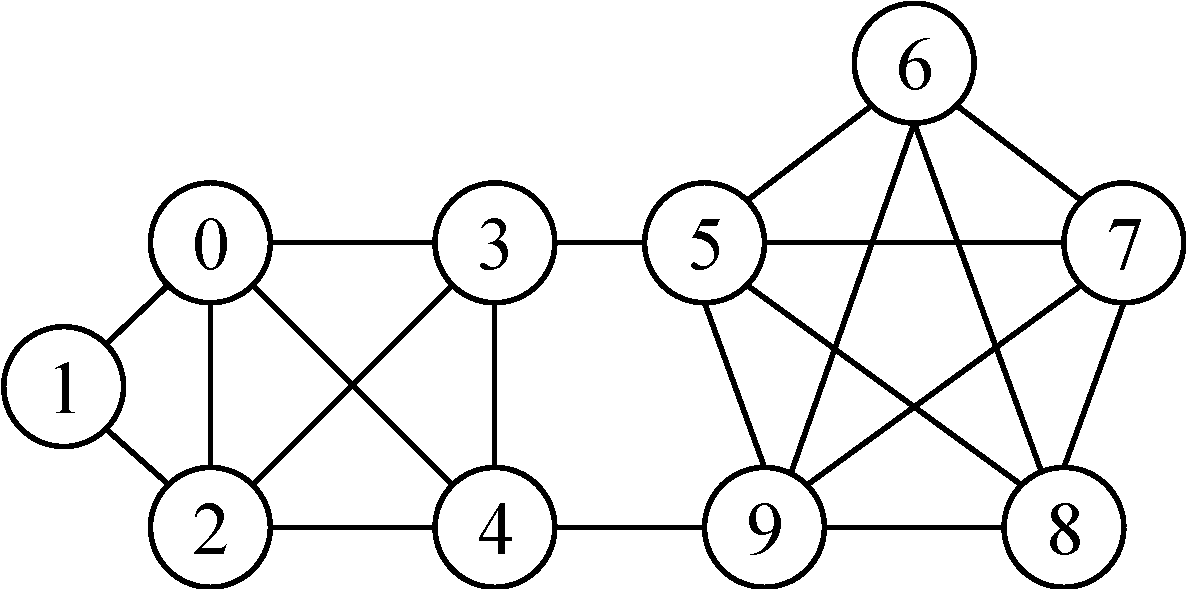
\includegraphics[width=1\linewidth,clip=true]{../img/graphs-Graph2.pdf}
    		(a)
    	\end{minipage}
    	\begin{minipage}{0.25\textwidth}
    		\centering
    		\[
	\begin{aligned}[t]
		C_{0} &: 0, 1, 2 \\
		C_{1} &: 0, 2, 3, 4 \\
		C_{2} &: 3, 5 \\
		C_{3} &: 5, 6, 7, 8, 9 \\
		C_{4} &: 4, 9
	\end{aligned}
\]

    		(b)
    	\end{minipage}
    	\begin{minipage}{0.15\textwidth}
    		\centering
    		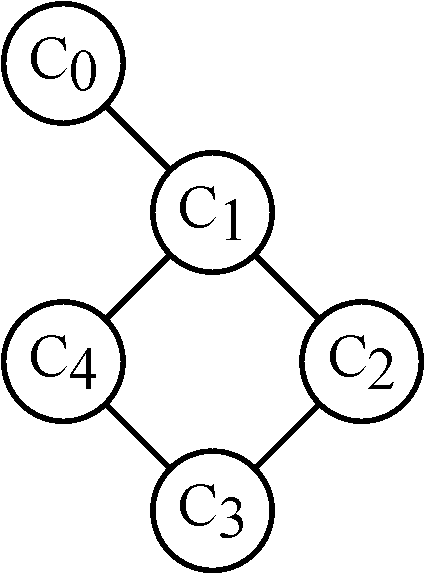
\includegraphics[width=1\linewidth,clip=true]{../img/graphs-Cliques2.pdf}
    		(c)
    	\end{minipage}
    \caption{(a) Grafo no dirigido. (b) Lista de cliques maximales. (c) Grafo de cliques.}
    \label{fig:gafoEj}
\end{figure}

\end{frame}



%% PARTICIONAR
\begin{frame}
\frametitle{Etapa 2: Particionar listado de cliques}

\begin{problem}
	\label{def:findPartitions}
	Encontrar particiones de cliques para el grafo de cliques $CG_{\mathcal{C}}$.
	
	Dado un grafo de cliques $CG_{\mathcal{C}} = (V_{\mathcal{C}}, E_{\mathcal{C}})$, encontrar un set de particiones de cliques $\mathcal{C}\mathcal{P} = \{cp_{1}, cp_{2}, ..., cp_{M}\}$ de $CG_{\mathcal{C}}(V_{\mathcal{C}}, E_{\mathcal{C}})$ con $M \geq 1$, tal que
	\begin{enumerate}
		%\item $\bigcup_{i \in \mathcal{C}\mathcal{P}} cp_{i} = CG_{i}$ \label{item:particiones1}
		\item $\bigcup\limits_{i = 1}^{M} cp_{i} = CG_{\mathcal{C}}$ \label{item:particiones1}
		\item $cp_{i} \cap cp_{j} = \varnothing$ para $i \neq j$ \label{item:particiones2}
		\item cualquier $cp_{i} \in \mathcal{C}\mathcal{P}$ es un subgrafo de $CG_{\mathcal{C}}(V_{\mathcal{C}}, E_{\mathcal{C}})$ inducido por el subset de vértices en $cp_{i}$ \label{item:particiones3}
	\end{enumerate}
	
\end{problem}

\end{frame}


\begin{frame}
\frametitle{Etapa 2: Algoritmo de particionamiento}

Definir una heurística que permita agrupar los cliques en particiones eficientes, que exploten su redundancia de vértices.

\begin{definition} 
	\label{def:rankingFunctions}
	Función de ranking
	
	Dado un grafo $G = (V, E)$ y $\mathcal{C} = \{c_{1}, c_{2}, ..., c_{N} \}$ el conjunto de tamaño $N$ de cliques maximales que cubren $G$, una función de ranking es una función $r: V \rightarrow \mathbb{R}^{+}$ que retorna un valor de puntuación para cada vértice $v \in V$.
\end{definition}

\end{frame}


\begin{frame}
\frametitle{Etapa 2: Algoritmo de particionamiento (2)}

Funciones de ranking propuestas, para $C(u) = \{c \in \mathcal{C}|u \in c\}$:

\begin{align}
	r_{f}(u) &= |C(u)| \label{eq:rankFunF}  \\ 
	r_{c}(u) &= \sum_{c \in C(u)}|c| \label{eq:rankFunC} \\ 
	r_{r}(u) &= \frac{r_{c}(u)}{r_{f}(u)} \label{eq:rankFunR}
\end{align}

%Complejidad: $O(L \log L)$; $L=\sum_{c_i \in \mathcal{C}}|c_{i}|$

\end{frame}


\begin{frame}
\frametitle{Etapa 2: Algoritmo de particionamiento (3)}

\begin{figure}
    	\centering
    	
    	\begin{minipage}{\textwidth}
    		\footnotesize
    		\centering
    		\[
	\begin{aligned}[t]
		C_{0} &: 0, 1, 2 \\
		C_{1} &: 0, 2, 3, 4 \\
		C_{2} &: 3, 5 \\
		C_{3} &: 5, 6, 7, 8, 9 \\
		C_{4} &: 4, 9
	\end{aligned}
\]

    	\end{minipage}
    	
    	\vspace{2mm}
    \begin{minipage}{\textwidth}
    		\footnotesize
    		\centering
    		\begin{tabular}{c|c|c|c|c|c|c|c|c|c|c|}
	\cline{2-11}
	$u \in G$ & 0 & 1 & 2 & 3 & 4 & 5 & 6 & 7 & 8 & 9 \\
	\cline{2-11}
	$R_{rf}$ & 2,0 & 1,0 & 2,0 & 2,0 & 2,0 & 1,0 & 1,0 & 1,0 & 1,0 & 2,0 \\
	\cline{2-11}
	$R_{rc}$ & 7,0 & 3,0 & 7,0 & 6,0 & 6,0 & 7,0 & 5,0 & 5,0 & 5,0 & 7,0 \\
	\cline{2-11}
	$R_{rr}$ & 3,5 & 3,0 & 3,5 & 3,0 & 3,0 & 3,5 & 5,0 & 5,0 & 5,0 & 3,5 \\
    \cline{2-11}
\end{tabular}

    \end{minipage}
    
    	\caption{Listado de cliques y puntajes de ranking asociados.}
    \label{fig:rankings}
\end{figure}

\end{frame}



\begin{frame}
\frametitle{Etapa 2: Algoritmo de particionamiento (4)}

\begin{algorithm}[H]
\caption{\footnotesize Algoritmo de particionamiento del grafo de cliques.}
\begin{algorithmic}[1]
\scriptsize
\REQUIRE $\mathcal{C}$ maximal clique collection ($N=|\mathcal{C}|$), ranking function $r(u)$
\ENSURE Returns clique-graph partition collection $\mathcal{C}\mathcal{P}$
\STATE $(D,R) \leftarrow computeRanking(r,\mathcal{C})$ (array $D$ y $R$, $\forall u \in V$ ) \label{alg:clustering:rankarray} 
\STATE Initialize bit array $Z$ of size $N$ and set each bit to 0
\FOR {$u \in R$}
    \STATE $cpid \leftarrow \emptyset$
     \FOR {$id \in D[u]$ and $Z[id]=0$} 
          \STATE $Z[id] \leftarrow 1$
          \STATE $cpid \leftarrow cpid \cup \{id\}$
    \ENDFOR
    \IF {$cpid \neq  \emptyset$}
      \STATE $\mathcal{C}\mathcal{P} \leftarrow \mathcal{C}\mathcal{P} : cpid$
    \ENDIF 
 \ENDFOR
\RETURN $\mathcal{C}\mathcal{P}$
\end{algorithmic}
\end{algorithm}

Complejidad: $O(N+V)$

\end{frame}		



\begin{frame}
\frametitle{Etapa 2: Algoritmo de particionamiento (5)}

\begin{figure}
    	\centering
    	
    	\begin{minipage}{\textwidth}
    		\footnotesize
    		\centering
    		\[
	\begin{aligned}[t]
		C_{0} &: 0, 1, 2 \\
		C_{1} &: 0, 2, 3, 4 \\
		C_{2} &: 3, 5 \\
		C_{3} &: 5, 6, 7, 8, 9 \\
		C_{4} &: 4, 9
	\end{aligned}
\]

    	\end{minipage}
    	
    	\vspace{2mm}
    	\begin{minipage}{\textwidth}
    		\footnotesize
    		\centering
    		\begin{tabular}{c|c|c|c|c|c|c|c|c|c|c|}
	\cline{2-11}
	$u \in G$ & 0 & 1 & 2 & 3 & 4 & 5 & 6 & 7 & 8 & 9 \\
	\cline{2-11}
	$R_{rf}$ & 2,0 & 1,0 & 2,0 & 2,0 & 2,0 & 1,0 & 1,0 & 1,0 & 1,0 & 2,0 \\
	\cline{2-11}
	$R_{rc}$ & 7,0 & 3,0 & 7,0 & 6,0 & 6,0 & 7,0 & 5,0 & 5,0 & 5,0 & 7,0 \\
	\cline{2-11}
	$R_{rr}$ & 3,5 & 3,0 & 3,5 & 3,0 & 3,0 & 3,5 & 5,0 & 5,0 & 5,0 & 3,5 \\
    \cline{2-11}
\end{tabular}

    	\end{minipage}
    	
    	\vspace{2mm}
    \begin{minipage}{\textwidth}
    		\footnotesize
    		\centering
    		\begin{tabular}{c|c|c|c|c|}
	\cline{2-5}
	$\mathcal{C}\mathcal{P}_{rf}$ & $C_{0} \quad C_{1}$ & $C_{2}$ & $C_{4}$ & $C_{3}$ \\
	\cline{2-5}
	$\mathcal{C}\mathcal{P}_{rc}$ & $C_{0} \quad C_{1}$ & $C_{2} \quad C_{3}$ & $C_{4}$ \\
	\cline{2-5}
	$\mathcal{C}\mathcal{P}_{rr}$ & $C_{3}$ & $C_{0} \quad C_{1}$ & $C_{2}$ & $C_{4}$ \\
	\cline{2-5}
\end{tabular}

    \end{minipage}
    
    	\caption{Particiones de cliques para cada función de ranking.}
    \label{fig:CPpartitions}
\end{figure}

\end{frame}




%% ESTRUCTURAS COMPACTAS
\begin{frame}
\frametitle{Etapa 3: Estructuras Compactas - Secuencias}

\begin{itemize}
	\item \textbf{X}: Listas concatenadas de vértices en $\mathcal{C}\mathcal{P}$.
	\item \textbf{B}: Bitmap indicando inicio de particiones.
	\item \textbf{BB}: Secuencia de bytes codificando presencia de vértices en cliques por partición.
	\item \textbf{Y}: Secuencia de enteros indicando primer byte en \textbf{BB} para cada partición.
\end{itemize}

\end{frame}


\begin{frame}
\frametitle{Etapa 3: Estructuras Compactas - Secuencias (2)}

\begin{figure}
    	\centering
    	
    	\begin{minipage}{\textwidth}
    		\footnotesize
    		\centering
    		\[
	\begin{aligned}[t]
		C_{0} &: 0, 1, 2 \\
		C_{1} &: 0, 2, 3, 4 \\
		C_{2} &: 3, 5 \\
		C_{3} &: 5, 6, 7, 8, 9 \\
		C_{4} &: 4, 9
	\end{aligned}
\]

    	\end{minipage}
    	
    	\vspace{2mm}
    	\begin{minipage}{\textwidth}
    		\footnotesize
    		\centering
    		\begin{tabular}{c|c|c|c|c|}
	\cline{2-5}
	$\mathcal{C}\mathcal{P}_{rr}$ &  $C_{0} \quad C_{1}$ & $C_{3}$ & $C_{2}$ & $C_{4}$ \\
	\cline{2-5}
\end{tabular}

    	\end{minipage}
    	
    	\vspace{2mm}
    \begin{minipage}{\textwidth}
    		\footnotesize
    		\centering
    		\begin{tabular}{c|c|c|c|c|c|c|c|c|c|c|c|c|c|c|c|}
	\cline{2-15}
	$X$: & 0 & 1 & 2 & 3 & 4 & 5 & 6 & 7 & 8 & 9 & 3 & 5 & 4 & 9 \\
	\cline{2-16}
	$B$: & 1 & 0 & 0 & 0 & 0 & 1 & 0 & 0 & 0 & 0 & 1 & 0 & 1 & 0 & 1 \\
	\cline{2-16}
	$BB$: & 3 & 1 & 3 & 2 & 2 \\
	\cline{2-6}
	$Y$: & 0 & 5 \\
	\cline{2-3}
\end{tabular}

    \end{minipage}
    
    	\caption{Secuencias finales.}
    \label{fig:sequences}
\end{figure}

\end{frame}



% ALGORITMOS
\begin{frame}
\frametitle{Algoritmos de consulta - Reconstrucción secuencial}

Recorre las particiones en orden secuencial.
\begin{itemize}
	\item Si contiene solo un clique, sus vértices son vecinos.
	\item Si no, se comparan los bytes de cada vértice entre si.
		\begin{itemize}
		\footnotesize
		\item Si la comparación es distinto a cero, son vecinos.
		\item No es necesario comparar siguientes bytes.
	\end{itemize}
\end{itemize}

\vspace{6mm}
Complejidad: 
$\begin{cases}
	O(P_{0} \cdot N^{2}), & bpu_{p} = 0 \\
	O(P_{1} \cdot N^{2} \cdot bpu_{p}), & bpu_{p} \neq 0  \\
\end{cases}$

\vspace{3mm}
{\footnotesize
$bpu_{p}$: Bytes por vértice de particiones.

$P_{0}$: Particiones que no tienen bytes por vértice.

$P_{1}$: Particiones que sí tienen bytes por vértice.

$N$: Largo de particiones.
}

\end{frame}


\begin{frame}
\frametitle{Algoritmos de consulta - Listado de vecinos}

Para un vértice $u$ aleatorio.
\begin{itemize}
	\item Cuenta ocurrencias de $u$ en $X$.
	\item Por cada una, se identifica su partición.
	\begin{itemize}
		\footnotesize
		\item Si contiene solo un clique, sus vértices son vecinos de $u$.
		\item Si no, se comparan sus bytes con los de cada posible vecino.
		\begin{itemize}
			\footnotesize
			\item Si la comparación es distinto a cero, son vecinos.
			\item No es necesario comparar siguientes bytes.
		\end{itemize}	
	\end{itemize}
\end{itemize}

\vspace{6mm}
Complejidad: 
$\begin{cases}
	O(M_{0} \cdot N), & bpu_{p} = 0 \\
	O(M_{1} \cdot N \cdot bpu_{p}), & bpu_{p} \neq 0  \\
\end{cases}$

\vspace{3mm}
{\footnotesize
$bpu_{p}$: Bytes por vértice de particiones.

$M_{0}$: Particiones que contienen a $u$ y no tienen bytes por vértice.

$M_{1}$: Particiones que contienen a $u$ y  sí tienen bytes por vértice.

$N$: Largo de particiones.
}

\end{frame}



\begin{frame}
\frametitle{Algoritmos de consulta - Vecindad de dos vértices}

Para dos vértices $u_{1}$, $u_{2}$ aleatorios.
\begin{itemize}
	\item Cuenta ocurrencias de ambos vértices en $X$.
	\item Revisa si coinciden en una partición
	\begin{itemize}
		\footnotesize
		\item Si coinciden, se comparan sus bytes.
		\begin{itemize}
			\footnotesize
			\item Si la comparación es distinto a cero, son vecinos.
			\item No es necesario comparar siguientes bytes.
		\end{itemize}
	\end{itemize}
\end{itemize}

\vspace{6mm}
Complejidad: 
$\begin{cases}
	O(M_{1} + M_{2}), & bpu_{p} = 0 \\
	O((M_{1} + M_{2}) \cdot bpu_{p}), & bpu_{p} \neq 0  \\
\end{cases}$

\vspace{3mm}
{\footnotesize
$bpu_{p}$: Bytes por vértice de particiones.

$M_{1}$: Particiones que contienen a $u_{1}$.

$M_{2}$: Particiones que contienen a $u_{2}$.
}

\end{frame}



\begin{frame}
\frametitle{Algoritmos de consulta - Cliques maximales}

Recorre las particiones en orden secuencial.
\begin{itemize}
	\item Si contiene un solo clique, lista sus vértices.
	\item Si no, se revisan los bytes de cada vértice ordenadamente.
	\begin{itemize}
		\footnotesize
		\item Si comparten un 1 en mismo bit, son un clique.
	\end{itemize}
\end{itemize}

\vspace{6mm}
Complejidad: 
$\begin{cases}
	O(P_{0} \cdot N), & bpu_{p} = 0 \\
	O(P_{1} \cdot N \cdot 8 \cdot bpu_{p}), & bpu_{p} \neq 0  \\
\end{cases}$

\vspace{3mm}
{\footnotesize
$bpu_{p}$: Bytes por vértice de particiones.

$P_{0}$: Particiones que no tienen bytes por vértice.

$P_{1}$: Particiones que sí tienen bytes por vértice.

$N$: Largo de particiones.
}

\end{frame}
